\chapter{Experimental Evaluation}
\label{ch:evaluation}
\chaptermark{Experimental Evaluation}

The experiments address construction and capacity (RQ1), execution (RQ2),
budget quality and reuse cost (RQ3), and competitive search regions (RQ4).

\section{Experimental Protocol}
\label{sec:7-1}

\subsection{Comparison protocol and reproducibility}

Datasets, timing and comparison families follow
\cref{sec:3-2,sec:3-3,sec:3-5}. The main RTX 5090 comparison measures
host-to-host steady-state throughput; construction and calibration are
timed separately. Ablation ratios retain their own family baselines.

Archived CPU JHQ results supply no matched-protocol CPU/GPU acceleration
factor: the October locality campaign uses Vogue with 1,024 lists and
level bits $[8,4]$, versus E1's 4,096 lists and different residual budget.
Older CSVs use a local reimplementation with documented legacy
recall-protocol issues.

Adaptive call counts and auxiliary device-only timing are documented in
\cref{sec:a-e1-protocol}.

Metrics and frontier estimators follow \cref{sec:3-2,sec:3-4};
$\glut$ and $\gscan$ retain the distinct meanings in \cref{sec:5-1}.





\section{Modern GPU ANN Recall--QPS Frontiers}
\label{sec:7-2}

\subsection{Comparison scope and frontier construction}

\Cref{fig:7-frontiers} compares JHQ-GPU with the graph, compressed-IVF
and brute-force baselines of \cref{sec:3-4} \cite{cagra,pq,ivfrabitq},
using the first four datasets in \cref{tab:3-data}. Each uses one batch
of 1,000 queries with common GT. T5 separately evaluates small batches
in \cref{sec:7-smallbatch}; \cref{sec:7-6} reports internal ablations.


The recorded schedule uses $\gscan=0$ for all 105 arXiv/OpenAI
run--budget cells and $\gscan=4$ for all 27 Vogue cells, triggered by
Vogue's candidate-count CV of 0.338--0.622. Thus the non-Vogue frontiers
exercise query-centric scanning, while Vogue also exercises grouped
retention, shared bounds and merging (\cref{sec:5-5}).

Applying the frontier rule in \cref{sec:3-4}, JHQ contributes 27--39
points per dataset and each baseline family 54--264. E1 contains 1,590
valid points, no failure records and no invalid-ID or duplicate-row flags.
These are parameter-sweep points, rather than independent index builds.


The tuning dimensions are listed in \cref{tab:3-grids}, with complete
coverage in \cref{sec:b-grids}. A curve ending before a target records
missing coverage of that finite grid.


\begin{figure}[tbp]
\centering
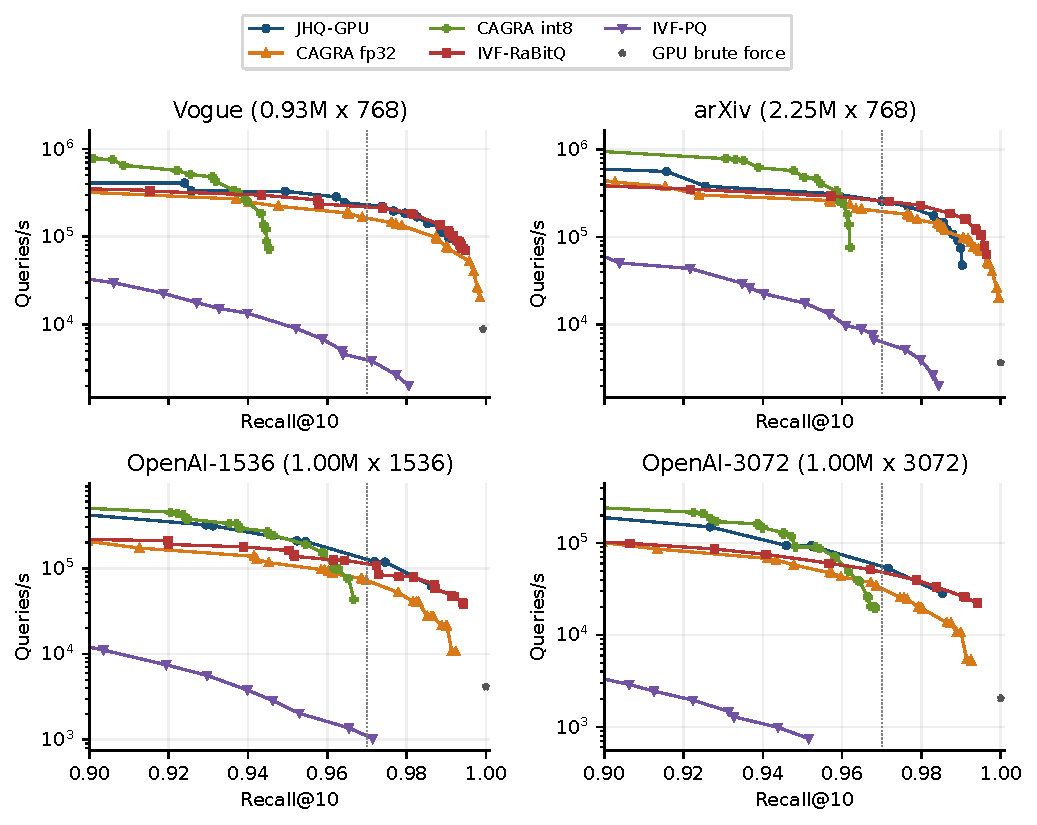
\includegraphics[width=\linewidth]{ch7/frontiers.pdf}
\caption[E1 recall--throughput frontiers]{Measured host-to-host recall--QPS frontiers on the four E1 datasets.
The displayed recall window begins at 0.90, with a vertical line at 0.97;
all baseline families,
including CAGRA int8, participate in frontier construction. Lines connect
measured points; throughput uses a logarithmic axis.}
\label{fig:7-frontiers}
\end{figure}

These curves are not memory-matched. Nine-bit RaBitQ has a nominal
$9d/8$ code budget comparable to JHQ, while its 4/8-bit arms use less.
\Cref{tab:4-bytes,sec:7-7} give representation costs and measured
allocations alongside this performance envelope.


\subsection{Matched recall and opposing operating regions}

\Cref{tab:7-matched} reports recall 0.97 using the interpolated and
qualifying-measured estimators defined in \cref{sec:3-4}.


\begin{table}[tbp]
\centering
\caption[Cross-system comparison at recall 0.97]{Recall 0.97 comparison. Each ratio is interpolated / measured;
values above one favour JHQ. JHQ kQPS is the interpolated estimate.
The small arXiv--RaBitQ difference changes direction with the estimator.}
\label{tab:7-matched}
\small\setlength{\tabcolsep}{4pt}
% Generated by scripts/build_ch7.py; do not edit numbers manually.
\begin{tabular}{@{}lrrr@{}}
\toprule
Dataset & JHQ kQPS & vs CAGRA fp32 & vs IVF-RaBitQ \\
\midrule
Vogue & 230.8 & 1.416 / 1.537 & 1.059 / 1.046 \\
arXiv & 258.6 & 1.317 / 1.422 & 0.996 / 1.015 \\
OpenAI-1536 & 126.7 & 1.747 / 2.294 & 1.130 / 1.111 \\
OpenAI-3072 & 55.9 & 1.747 / 2.088 & 1.157 / 1.346 \\
\bottomrule
\end{tabular}

\end{table}

At recall 0.97, JHQ's interpolated rate is $1.317$--$1.747\times$
CAGRA fp32's. It also leads IVF-RaBitQ on three datasets; arXiv is a
near tie whose direction changes with the estimator (\cref{tab:7-matched}).
Grid spacing matters: OpenAI-1536's CAGRA comparison is $1.747\times$
by interpolation and $2.294\times$ at qualifying measured points.

Vogue's lead depends on the grouped execution path. Replacing it by
$\gscan=0$ changes the recall-0.97 ratio against RaBitQ from $1.059$
to $0.933$ on the same batch-1,000 grid. Each pair fixes the index,
probes, budget and final outputs. This links RQ2 to RQ4 through the
integrated path, without isolating the shared bound alone.

The advantage changes with the recall target. CAGRA int8 is about
$1.20$--$1.98\times$ faster at 0.90--0.92 but has no qualifying point
at 0.97 in these grids. IVF-RaBitQ regains the lead at several targets
of 0.98 or above; CAGRA fp32 also leads on arXiv near 0.99.
\Cref{fig:7-frontiers} therefore supports a high-recall operating region,
with both the competitor's precision and measured coverage specified.

\subsection{Precision sensitivity on the OpenAI datasets}
\label{sec:7-precision}

Supplementary source inspection establishes that the E1 implementation
uses TF32 multiplication with FP32 accumulation for OpenAI rotation and
centroid GEMMs, despite FP32 input/storage and a misleading source comment
(\cref{sec:4-2}). The main E1 frontier remains the historical measurement
of that implementation. A separate FP32 variant changes the cuBLAS
math-mode switch and replays 37/39 OpenAI configurations at batch 1,000,
five rounds each. Execution order alternates between variants across
probe settings. Both reuse the same TF32-trained model; the intervention
changes add/query arithmetic, including database encoding and routing.
It is not a comparison of independently FP32-trained models.
\Cref{tab:7-precision} summarises the paired changes.

\par\medskip\noindent\begin{minipage}{\linewidth}
\centering\captionsetup{hypcap=false}
\captionof{table}[FP32 sensitivity at matched configurations]{FP32 sensitivity. QPS ratio is FP32/TF32 at equal configuration
(geometric mean); recall differences have the same direction. The last
two columns compare the FP32 frontier at recall 0.97 with archived E1
IVF-RaBitQ and CAGRA fp32 frontiers. Baselines were not remeasured.}
\label{tab:7-precision}
\scriptsize\setlength{\tabcolsep}{3pt}
\begin{tabular}{@{}lrrrrr@{}}
\toprule
Dataset & Pairs & QPS ratio & $\Delta$Recall & vs RaBitQ & vs CAGRA \\
\midrule
OpenAI-1536 & 37 & 0.953 & +0.0003--+0.0005 & 1.086 & 1.679 \\
OpenAI-3072 & 39 & 0.951 & +0.0000--+0.0003 & 1.079 & 1.629 \\
\bottomrule
\end{tabular}

\end{minipage}\par\medskip

At equal configuration, FP32 reduces throughput by about 5\% and increases
recall by 0--0.0005. At matched recall 0.97, its throughput is about 3\%
below the same-session TF32 frontier. It remains $1.086\times$ and
$1.079\times$ archived RaBitQ, and $1.679\times$ and $1.629\times$
archived CAGRA fp32. Same-session v69/RaBitQ ratios are 1.118/1.114,
versus historical 1.130/1.157. This separates the precision intervention
from session variation: the competitive direction persists, with smaller
margins, while the cross-session baseline comparison retains timing
uncertainty. The two precision variants' complete frontiers are shown in
\cref{fig:7-precision}.

\begin{figure}[tbp]
\centering
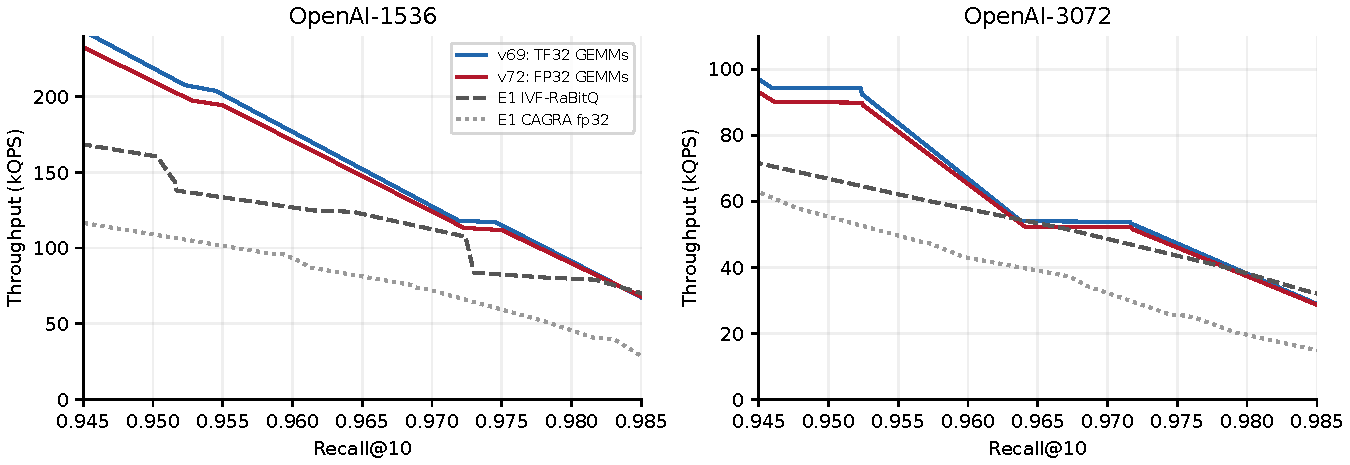
\includegraphics[width=\linewidth]{supplement/precision.pdf}
\caption[TF32 and FP32 precision frontiers]{Supplementary precision frontiers. Solid curves are same-session
JHQ variants; dashed/dotted baselines are historical E1 measurements.
All use the chapter's frontier and interpolation rules.}
\label{fig:7-precision}
\end{figure}


\subsection{Interpretation and comparison limits}

The OpenAI pair supplies a row-aligned embedding-width contrast from
Qdrant's DBpedia \texttt{text-embedding-3-large} corpus family
\cite{data_openai1536,data_openai3072}. The supplementary check compares
all 1,000 query rows and every 97th base row (10,299 rows): truncating
and renormalising the 3,072-dimensional vector gives cosine at least
0.9980 against its 1,536-dimensional counterpart, with median 1.000000.
GT top-10 overlap averages 9.046/10. This strongly supports matching row
order in the inspected exports; original entity-ID mappings were not
exported. Doubling dimension leaves the historical 0.97 CAGRA fp32
ratio at 1.747 in both datasets and changes the RaBitQ ratio from
1.130 to 1.157. The FP32 sensitivity likewise retains comparable
advantages. Dimension alone therefore does not explain the observed
advantage within this paired corpus/embedding contrast.

The four-dataset advantage co-varies with the 128-probe refinement
anchors: 4--8 for OpenAI, 64 for Vogue and 100 for arXiv
(the later FULL rule selects 200 there). These anchors are not the
matched-recall frontier parameters, so the association does not isolate
primary quality causally.

The interface, memory and compilation differences in \cref{sec:3-3}
remain relevant to small margins. \Cref{sec:7-8} examines their empirical
sensitivity.


\subsection{Small batches change the competitive region}
\label{sec:7-smallbatch}

T5 compares scheduled JHQ, CAGRA fp32/int8 and IVF-RaBitQ at batches
8/32 on the four E1 datasets. Five synchronous host-to-host rounds use
1,000/992 queries, respectively. Its 1,808 points include JHQ's one-block
control; IVF-PQ and brute force are outside this campaign.
\Cref{fig:7-smallbatch,tab:7-smallbatch} compare the resulting regions.

\suppressfloats[t]
\begin{figure}[htbp]
\centering
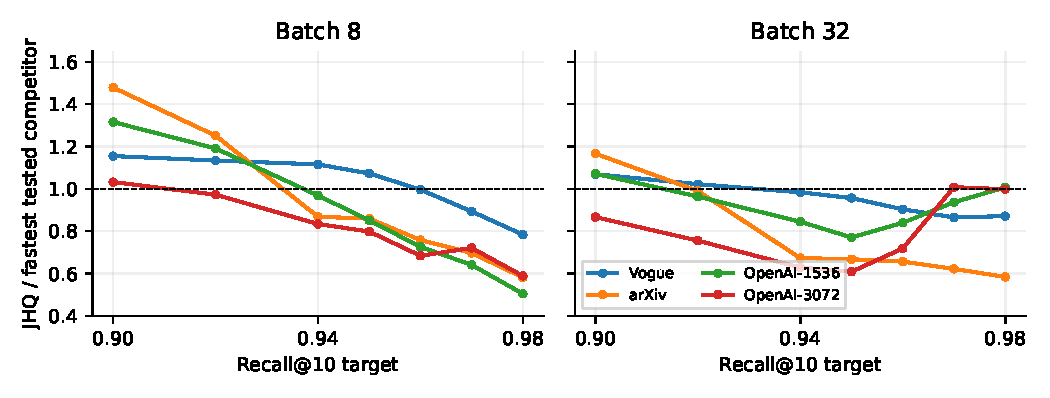
\includegraphics[width=\linewidth]{t4-t5/smallbatch.pdf}
\caption[Small-batch competitive regions]{T5 JHQ / fastest-competitor
QPS under interpolation with qualifying measured endpoints. Above one
favours JHQ. Strict measured thresholds are in \cref{tab:7-smallbatch}.}
\label{fig:7-smallbatch}
\end{figure}

\begin{table}[htbp]
\centering
\caption[Small-batch matched-recall ratios]{T5 QPS ratios:
interpolation with qualifying endpoints / strict measured threshold.
The fastest competitor is selected independently for each estimator;
higher-recall qualifying endpoints remain eligible without extrapolation.}
\label{tab:7-smallbatch}
\footnotesize\setlength{\tabcolsep}{4pt}
\begin{tabular}{@{}lrrrr@{}}
\toprule
Dataset & $b$ & $R=0.90$ & $R=0.95$ & $R=0.97$ \\
\midrule
Vogue & 8 & 1.155 / 1.091 & 1.073 / 0.980 & 0.893 / 0.854 \\
Vogue & 32 & 1.069 / 0.997 & 0.956 / 0.895 & 0.865 / 0.839 \\
arXiv & 8 & 1.479 / 1.454 & 0.859 / 0.851 & 0.697 / 0.698 \\
arXiv & 32 & 1.166 / 1.148 & 0.667 / 0.661 & 0.622 / 0.582 \\
OpenAI-1536 & 8 & 1.316 / 1.131 & 0.851 / 0.825 & 0.641 / 0.620 \\
OpenAI-1536 & 32 & 1.071 / 0.915 & 0.770 / 0.752 & 0.937 / 0.914 \\
OpenAI-3072 & 8 & 1.032 / 0.953 & 0.798 / 0.798 & 0.721 / 0.702 \\
OpenAI-3072 & 32 & 0.866 / 0.734 & 0.608 / 0.771 & 1.008 / 1.351 \\
\bottomrule
\end{tabular}

\end{table}

At recall 0.97 and batch 8, CAGRA fp32 leads on all four datasets under
both estimators: interpolated JHQ ratios are 0.641--0.893. At batch 32,
these ratios are 0.622--1.008, with OpenAI-3072 close under interpolation
but favourable to JHQ under the measured threshold. At recall 0.95,
Vogue's batch-8 lead likewise appears only under interpolation. Grid
resolution therefore matters to borderline rankings.

Lower-recall comparisons must retain competitors whose fastest frontier
point already exceeds the target.
At 0.90, corrected interpolated ratios are 1.032--1.479 at batch 8 and
0.866--1.166 at batch 32; the strict measured estimator gives three
and one JHQ wins, respectively. Omitting qualifying endpoints would
overstate these low-recall leads.
Scheduling is still useful: at recall 0.95 its interpolated gain over
one block is 1.7--3.3$\times$. An internal execution gain therefore need
not produce a cross-system lead.

Null-call medians by dataset, method and batch span 0.012--0.072\,ms;
this overhead remains in search timing. CAGRA uses Python bindings, while JHQ/RaBitQ use C++;
warm-up policies also differ. Protocol and grid details are in \cref{sec:a-t4-t5}. E1's full-batch
high-recall leads do not generalise to these small batches.


\section{Cartesian LUT, Packed Loads and Lane Refinement}
\label{sec:7-3}

The RQ2 ablations measure both kernel and application effects.

\subsection{Exact table factorization and its throughput consequence}

The LUT ablation tests the cost model in \cref{sec:5-2} and FP32 ranking
effects.


\Cref{fig:7-lut} compares Cartesian table grouping on six datasets,
probe counts 8/32/128/512,
fixed $\alpha=100$, and $\glut\in\{1,2,4,8\}$. Each arm has five timing
rounds; batch size is 1,000 except Stella's 999 queries. Two groups have
the highest median throughput in 22 of 24 cells. The exceptions are
arXiv at 128 probes, where one group is about 0.23\% faster, and
OpenAI-3072 at eight probes, where four groups are about 0.84\% faster.
These narrow differences are best treated as near ties. The newer count
is 22/24, rather than the historical ADC paper's 23/24.
In the specific two-group versus one-group comparison, two groups win
23/24 cells; each dataset's four-probe geometric-mean ratio exceeds one
(1.021--1.318). This supports the choice across the tested workloads
without treating configurations sharing an index as independent trials.

\begin{figure}[tbp]
\centering
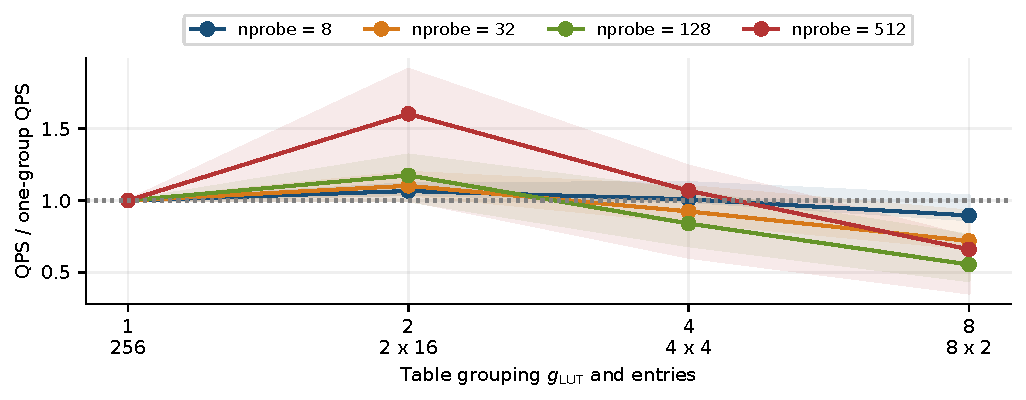
\includegraphics[width=\linewidth]{ch7/lutgroups.pdf}
\caption[Cartesian lookup-table grouping]{Cartesian table grouping at fixed $\alpha=100$ (v71).
Group counts describe $\glut$, not parallel scan groups. Curves are medians
of per-dataset QPS ratios to the one-group arm; shading shows their range.}
\label{fig:7-lut}
\end{figure}

The two-group/one-group ratio ranges from $0.998$ to $1.914$.
Four and eight groups each store 16 entries but require more lookups
and additions. These arms show that smaller tables need not improve
throughput; occupancy and instruction costs were not isolated. The maximum
reported recall spread within any four-arm cell is $10^{-4}$.
At 128 probes and $\alpha=100$, T4 compares identical candidates on
Vogue, arXiv and OpenAI-3072. Full versus $16+16$ tables differ in
22.6--26.1\% of candidate-score bit patterns, with maximum relative error
$4.53\times10^{-7}$. Across all forms, 20.5--29.4\% differ, with maximum
relative error $4.64\times10^{-7}$. Vogue has 2--4/256 final-ID
differences, while arXiv/OpenAI have none. Unchanged primary survivor
sets can still produce different final IDs because the rounded primary
score enters refinement (\cref{sec:a-t4-t5}).


\subsection{Packed access and cooperative residual scoring}

The historical packing experiment compares byte-oriented and word-oriented
access while holding the dataset, probe count and table grouping fixed.
Across six datasets, four probe counts and $\glut\in\{1,2\}$, the 48
pairs yield throughput ratios from $1.012$ to $1.658$, with maximum recall
difference $10^{-4}$. Gains are generally smaller at eight probes and
larger at 512. Both alternatives already use a subspace-major layout;
this experiment supports packed access, not a claim that a physical
transpose alone produced the improvement. Each arm has one reported
aggregate rate, so this older evidence has weaker uncertainty information
than the five-round v71 sweep.

\Cref{fig:7-packing-refinement,tab:7-refinement} then separate wider loads
from lane cooperation in residual refinement. L0 is the original scalar
path; L1 changes the load path without distributing a candidate across
multiple lanes; L16 assigns 16 lanes to a candidate. The same process
rotates arm order across five timing rounds, with three search calls per
arm per round. For the twelve ordinary configurations, L16 improves
end-to-end throughput by $1.015$--$1.789\times$. An additional arXiv
configuration at $\alpha=200$, explicitly a high-budget control, reaches
$2.383\times$; it is not the gain range of the ordinary selected budgets.

\begin{figure}[tbp]
\centering
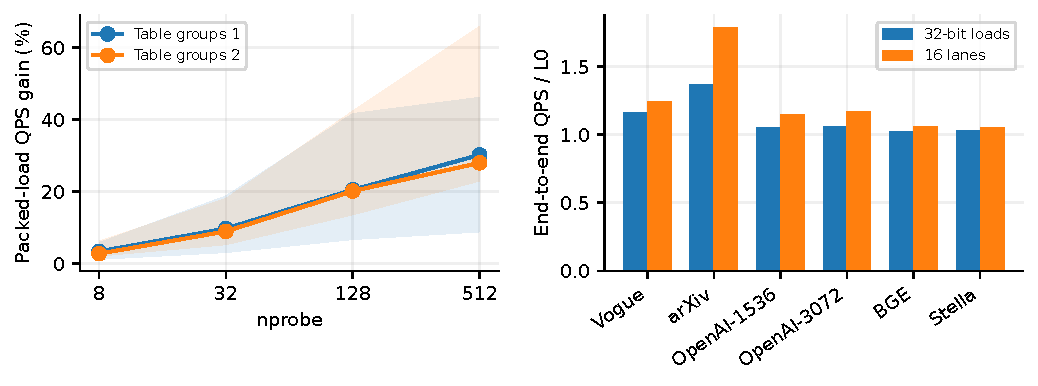
\includegraphics[width=\linewidth]{ch7/packing_refinement.pdf}
\caption[Packed access and refinement controls]{Packing and refinement controls. Left: median packed-load QPS
 gain across six datasets, with shaded minimum--maximum ranges, for each
 table grouping and probe count. Right: measured load-only and 16-lane
 end-to-end gains at 128 probes and the ordinary dataset-specific budgets.
 These panels come from different experiment families.}
\label{fig:7-packing-refinement}
\end{figure}

\begin{table}[tbp]
\centering
\caption[Refinement gains at 128 probes]{Refinement at 128 probes. Ratios are paired end-to-end gains over
 L0, except the last column, which is the profiled refinement-kernel gain.
 The kernel and application gains must not be interchanged.}
\label{tab:7-refinement}
\small\setlength{\tabcolsep}{4pt}
% Generated by scripts/build_ch7.py; do not edit numbers manually.
\begin{tabular}{@{}lrrrr@{}}
\toprule
Dataset & $\alpha$ & $L1/L0$ QPS & $L16/L0$ QPS & Kernel gain \\
\midrule
arXiv & 100 & 1.368 & 1.789 & 5.97 \\
BGE & 32 & 1.026 & 1.062 & 1.97 \\
OpenAI-1536 & 8 & 1.055 & 1.145 & 3.34 \\
OpenAI-3072 & 4 & 1.063 & 1.171 & 8.81 \\
Stella & 16 & 1.030 & 1.053 & 2.66 \\
Vogue & 64 & 1.161 & 1.240 & 3.72 \\
\bottomrule
\end{tabular}

\end{table}

The load-only control is bit-identical to L0 in the tested cases, yet
already improves arXiv throughput by $1.368\times$. Lane cooperation adds
a larger reduction in refinement time. On arXiv at $\alpha=100$, the
profiled refinement kernel falls from 4,277.5 to 716.8\,$\mu$s, a
$5.97\times$ gain, while total throughput improves $1.789\times$.
OpenAI-3072's refinement kernel improves $8.81\times$, but total throughput
improves $1.171\times$. The remaining routing, screening, selection and
transfer costs limit the application gain.

A quantitative Amdahl check uses the refinement kernel's baseline time
as a fraction $f$ of host-to-host baseline latency and its kernel speedup
$s$, giving $1/(1-f+f/s)$ if the remaining time is unchanged. The fractions
are approximately 0.529 on arXiv and 0.168 on OpenAI-3072, producing
estimates of $1.787\times$ and $1.175\times$, close to the measured
$1.789\times$ and $1.171\times$. These combine separate kernel-profile
and wall-time measurements and are explanatory estimates.

Cooperative reductions alter floating-point addition order. The tested
multi-lane variants have very small distance differences, with maximum
reported relative error about $1.6\times10^{-6}$, and occasional changes
near ranking boundaries. Sanitizer checks cover the recorded refinement
and top-$k$ kernels on small query subsets. These checks and numerical
tolerances delimit the evidence; multi-lane scoring is not universally
bit-identical.

\section{Global Top-c, Shared Bound and Probe Correctness/Ablation}
\label{sec:7-4}

The representation checks in \cref{sec:4-6} concern the stored index;
this section evaluates query selection and its cost.


\subsection{Strict CPU reference for computed-score selection}
\label{sec:7-strict-selection}

The supplementary T4 campaign sorts every visited candidate on the CPU
under $(\primarydist,\mathrm{position})$, using GPU-produced FP32 scores.
Its diagnostic exporter follows the packed scan layout and accumulation
order; exported scores match all returned valid primary scores bit for
bit. Source comparison confirms that the diagnostic version changes only
export, relative to the table-sweep implementation.
Vogue, arXiv and OpenAI-3072 are tested at 1/8/128 probes,
$\alpha\in\{4,100,200\}$, $\gscan\in\{0,1,2,4,8\}$ and both shared-bound
settings: 270 configurations of 256 queries, or 69,120 query instances
(\cref{tab:7-strict-selection}).

\suppressfloats[t]
\begin{table}[htbp]
\centering
\caption[Strict computed-score selection checks]{T4 CPU-reference checks.
Set and order equality use the complete primary key. Valid count checks
$\min(c,n_c)$ survivors; final equality sorts retained computed refined
scores by $(\refineddist,\mathrm{ID})$, including their FP32 bits. Counts
are query instances, with queries reused across configurations.}
\label{tab:7-strict-selection}
\footnotesize\setlength{\tabcolsep}{3pt}
\begin{tabular}{@{}lrrrrr@{}}
\toprule
Path & Queries & Set / order exact & Tie-only & Valid count & Final exact \\
\midrule
$\gscan\geq1$ & 55,296 & 55,296 / 55,296 & 0 & 55,296 & 55,296 \\
$\gscan=0$ & 13,824 & 13,768 / 8,758 & 56 & 13,824 & 13,824 \\
\bottomrule
\end{tabular}

\end{table}

All 55,296 grouped instances match the complete-key reference in order.
The one-block path satisfies the distance preorder in all 13,824 instances;
its 56 set differences are exclusively cutoff ties. There are 19,120
underfull instances with the correct number of valid survivors, and all
69,120 final selections match the retained-score reference.
This directly tests the stage contracts of
\cref{lem:5-buffer,prop:5-local-coverage,prop:5-shared-bound}.
The earlier 64 scan comparisons and 48 shared-bound comparisons provide
separate paired-implementation evidence; archived sanitizer runs cover
smaller subsets. Export and retention details are in \cref{sec:a-t4-t5}.


\subsection{Shared bounds preserve the selection target}

\Cref{prop:5-shared-bound} establishes the selection guarantee. The
paired experiment measures the work saved by sharing that bound.


Across four workloads and four batch sizes, all 48 shared-bound versus
independent-bound comparisons agree on primary and final outputs.
Five-round paired throughput ratios span $0.994$--$1.562\times$.
On arXiv at $\alpha=200$, batch 1,000 and eight groups, the paired
profile reduces merge time from about 2,629 to 471\,$\mu$s and scan
from 7,968 to 5,513\,$\mu$s. Sharing therefore reduces intermediate work
in suitable workloads, with small regressions elsewhere.

The rejected static-quota design faces concentrated winners: the first
candidate group holds 46--81\% of global survivors in the pilot workloads.
Equal quotas would require a correctness fallback; calibrated unequal
quotas leave the dominant group on the critical path. These observations
motivate shared bounds within that pilot's scope.

\subsection{Exact probe selection and the limits of pipeline identity}

Once screening becomes faster, IVF probe selection becomes a larger
fraction of small-batch time. The radix probe primitive (v69) changes how the
smallest computed centroid scores are selected while retaining the
preceding score arithmetic. On OpenAI this includes TF32 GEMMs
(\cref{sec:7-precision}).
Its synthetic checker covers 1,792 cases and reports zero failures.
Checks of the real arXiv, Vogue and OpenAI-3072 workloads find identical
probe identifiers and identical primary top-$c$ positions and distances
for all 1,000 queries.

\begin{table}[tbp]
\centering
\caption[Probe-selection throughput ratios]{v69/v65 end-to-end throughput ratios for the exact computed-score probe
 change. Each workload--batch comparison has ten timing rounds per binary,
 collected in alternating runs. Values above one favour v69.}
\label{tab:7-probe}
\small
% Generated by scripts/build_ch7.py; do not edit numbers manually.
\begin{tabular}{@{}lrrrr@{}}
\toprule
Dataset & Batch 8 & 32 & 256 & 1,000 \\
\midrule
arXiv & 1.074 & 1.063 & 1.035 & 1.034 \\
Vogue & 1.109 & 1.103 & 1.052 & 1.041 \\
OpenAI-3072 & 1.167 & 1.117 & 1.055 & 1.050 \\
\bottomrule
\end{tabular}

\end{table}

\Cref{tab:7-probe} shows end-to-end improvements of $1.034$--$1.167\times$.
At batch 8, the profiled probe stage falls from 56.5 to 22.6\,$\mu$s
on arXiv, 52.7 to 14.7\,$\mu$s on Vogue, and 77.8 to 16.7\,$\mu$s
on OpenAI-3072. The unchanged stages limit full-batch gains. These
within-family ratios have different baselines from the preceding ablations.

On Vogue, the probe/primary dump is
byte-identical across the two binaries for all 1,000 queries in the
one-group, batch-8 test, yet final recall is 0.9642 versus 0.9644. The
same baseline binary also changes from 0.9642 in the identity run to
0.9644 in each of its two timing runs. The variation therefore also
occurs without the probe change and lies after primary selection in the
dump-controlled case. Its root cause remains unresolved. Scheduled and
one-block outputs are bit-identical within each checked process; dump
coverage is in \cref{app:reproducibility}.

Finally, the optional v70 FP16 experiment is a separate approximation.
Its probe sets match the v69 reference on 936/1,000 arXiv queries, 979/1,000
Vogue queries and 998/1,000 OpenAI-3072 queries, with very high mean
set overlap. High overlap and small recall changes do not make the
primitive exact. Those results are excluded from the main E1 frontier
and from the exact-probe claim.

\section{Held-out Budget Quality, Throughput and Payback}
\label{sec:7-5}

RQ3 compares the policy of \cref{ch:refinement} with fixed
$\alpha=100$ and the stronger universal control $\alpha=64$.

\subsection{Unlabelled selection and a labelled diagnostic oracle}

The six datasets are tested at 128 and 512 probes with the fixed,
sampled, FULL, enumeration and oracle controls in \cref{sec:6-4}.
The disjoint pools and 64 draws per sample size follow \cref{sec:3-2}.


All rule variants use \cref{eq:6-agreement} with $k=10$ and $\epsilon=1$.
FULL uses all calibration queries; the diagnostic oracle uses held-out
labels (\cref{tab:6-controls}).


\subsection{Full-pool calibration as the quality-first working point}

Full-pool calibration uses all 500 calibration queries once per cell.
Its selected arms meet the held-out $10^{-3}$ loss target in 12/12 cells;
the largest observed loss is 0.0006. Their rates are 0.908--1.000 of the
GT oracle's, and calibration costs 9.5--60.3\,ms. The geometric-mean
rate ratio to fixed 100 is $1.111\times$, or $1.193\times$ over the ten
cells where fixed 100 also meets the target. \Cref{tab:7-budget-full}
shows the complete comparison. Against fixed 64, full-pool selection is
faster in six cells, equal in two and slower in four: its main advantage
is the observed coverage of all twelve quality targets.

These cells favour FULL for quality coverage and $S=128$ for lower
calibration cost, within the statistical scope of \cref{sec:6-2}.


\begin{table}[tbp]
\centering
\caption[Full-pool budget calibration]{Full-pool calibration ($S=500$). Loss is relative to the best
measured held-out recall; rates are kQPS from the selected fixed arm.
``Cal.'' is one full-pool calibration call per cell, not a repeated
stream timing. Held-out counts are 500, or 499 for Stella.}
\label{tab:7-budget-full}
\footnotesize\setlength{\tabcolsep}{3pt}
% Generated by scripts/build_ch7.py; do not edit numbers manually.
\begin{tabular}{@{}lrrrrrrr@{}}
\toprule
Dataset & Probe & $\alpha_{\rm full}$ & Loss & $Q_{\rm full}$ & vs 100 & vs oracle & Cal. ms \\
\midrule
Vogue & 128 & 100 & 0.0000 & 202.9 & 1.000 & 0.908 & 10.1 \\
arXiv & 128 & 200 & 0.0000 & 151.5 & 0.728 & 1.000 & 10.0 \\
OpenAI-1536 & 128 & 8 & 0.0000 & 267.7 & 1.599 & 1.000 & 9.5 \\
OpenAI-3072 & 128 & 4 & 0.0000 & 145.0 & 1.691 & 1.000 & 17.1 \\
BGE & 128 & 64 & 0.0006 & 124.9 & 1.075 & 0.932 & 17.1 \\
Stella & 128 & 16 & 0.0006 & 110.4 & 1.153 & 1.000 & 20.6 \\
Vogue & 512 & 100 & 0.0002 & 100.1 & 1.000 & 0.969 & 20.9 \\
arXiv & 512 & 200 & 0.0000 & 69.0 & 0.831 & 1.000 & 25.1 \\
OpenAI-1536 & 512 & 8 & 0.0000 & 114.9 & 1.326 & 1.000 & 21.8 \\
OpenAI-3072 & 512 & 4 & 0.0002 & 52.1 & 1.219 & 0.977 & 40.5 \\
BGE & 512 & 64 & 0.0006 & 50.8 & 1.033 & 1.000 & 42.3 \\
Stella & 512 & 16 & 0.0006 & 36.0 & 1.041 & 1.000 & 60.3 \\
\bottomrule
\end{tabular}

\end{table}

\subsection{Lower-cost sampling and its quality risk}

\Cref{tab:7-budget-quality} reports the $S=128$ result. The median selected
budget matches the oracle budget in ten of twelve cells; it differs on
arXiv at 128 probes and OpenAI-3072 at 512. The selected budgets span
4--200, indicating substantial workload dependence. Median budget and
mean recall need not describe one arm. The latter is reconstructed from
printed best recall minus mean loss and is approximate at four decimals.

\begin{table}[tbp]
\centering
\caption[Sampled-budget held-out quality]{Held-out quality at $S=128$. Rule $\alpha$ is the median across
64 draws; oracle $\alpha$ uses held-out labels. $\overline R_{\rm rule}$
is reconstructed mean recall. ``Losses'' counts draws with recall loss
$>10^{-3}$ relative to the best tested held-out recall; $L_{95}$ is the
logged lower-order 95th-percentile loss estimate. $R_{100}$ is
fixed-budget recall.}
\label{tab:7-budget-quality}
\small\setlength{\tabcolsep}{3pt}
% Generated by scripts/build_ch7.py; do not edit numbers manually.
\begin{tabular}{@{}lrrrrrr@{}}
\toprule
Dataset & Probe & $\alpha$: rule/oracle & $R_{100}$ & $\overline{R}_{\rm rule}$ & Losses & $L_{95}$ \\
\midrule
Vogue & 128 & 64 / 64 & 0.9680 & 0.9677 & 5/64 & 0.0022 \\
arXiv & 128 & 100 / 200 & 0.9748 & 0.9751 & 40/64 & 0.0024 \\
OpenAI-1536 & 128 & 8 / 8 & 0.9280 & 0.9279 & 4/64 & 0.0000 \\
OpenAI-3072 & 128 & 4 / 4 & 0.9252 & 0.9252 & 0/64 & 0.0000 \\
BGE & 128 & 32 / 32 & 0.9198 & 0.9190 & 1/64 & 0.0008 \\
Stella & 128 & 16 / 16 & 0.9892 & 0.9884 & 6/64 & 0.0030 \\
Vogue & 512 & 64 / 64 & 0.9916 & 0.9915 & 2/64 & 0.0002 \\
arXiv & 512 & 200 / 200 & 0.9878 & 0.9885 & 32/64 & 0.0016 \\
OpenAI-1536 & 512 & 8 / 8 & 0.9740 & 0.9738 & 4/64 & 0.0000 \\
OpenAI-3072 & 512 & 4 / 8 & 0.9704 & 0.9702 & 0/64 & 0.0002 \\
BGE & 512 & 64 / 64 & 0.9670 & 0.9661 & 24/64 & 0.0014 \\
Stella & 512 & 16 / 16 & 0.9954 & 0.9945 & 7/64 & 0.0030 \\
\bottomrule
\end{tabular}

\end{table}

ArXiv exposes the sampling risk: 40/64 draws at 128 probes and 32/64
at 512 exceed the $10^{-3}$ loss threshold, despite mean loss 0.0009
in both cells. Fixed 100 itself loses 0.0012/0.0016, so improvement
over that default coexists with failure against the stronger target.
Other tails are in \cref{tab:7-budget-quality}: BGE/512 has 24/64
crossings and $L_{95}=0.0014$; Stella has $L_{95}=0.0030$ at both
probe depths, while OpenAI-3072 has no observed crossings.
Under the percentile convention in \cref{sec:a-budget-contract},
four nonzero losses can coexist with $L_{95}=0$, as on OpenAI-1536.

\begin{figure}[tbp]
\centering
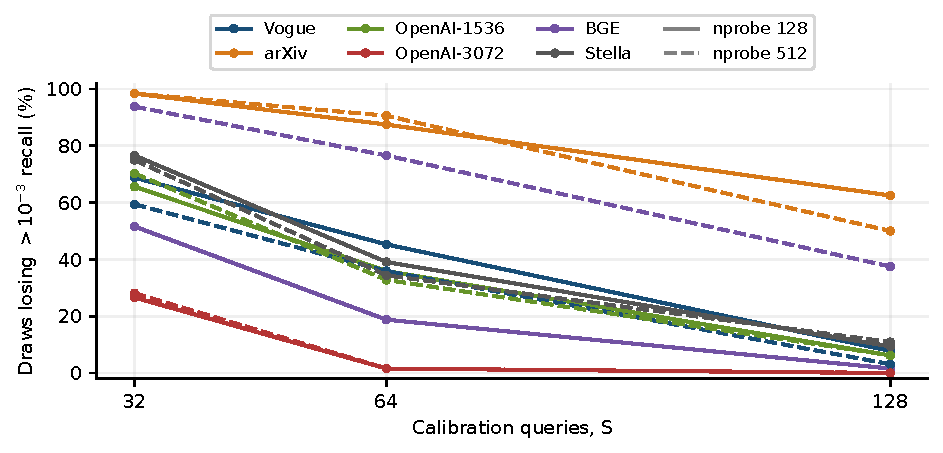
\includegraphics[width=0.82\linewidth]{ch7/budget_risk.pdf}
\caption[Held-out risk across sample sizes]{Held-out risk across sample sizes. The vertical axis is the
percentage of calibration draws losing more than $10^{-3}$ held-out recall
relative to the best tested budget. Increasing $S$ also tightens the allowed
slot-disagreement fraction because \cref{eq:6-agreement} keeps threshold one.}
\label{fig:7-budget-risk}
\end{figure}

Increasing $S$ tightens the normalised allowance $1/(10S)$ as well
as changing sample coverage (\cref{fig:7-budget-risk}).
The grouped-path guarantee covers 2,176/2,304 sampled draws;
the remaining 128 distance-only cases are empirical checks
(\cref{cor:6-grouped-calibration}). Enumeration and FULL verification
are reported in \cref{sec:7-budget-trace}.

Fixed 64 and fixed 100 each meet the diagnostic quality target in 10/12
cells; fixed 200 meets it in all twelve. FULL selects 100 on Vogue
where the fastest qualifying oracle arm is 64: minimum reference
disagreement and maximum quality-constrained throughput are different
objectives. The observed low-budget timing plateau reinforces this
distinction.

\subsection{Estimated throughput and calibration economics}

Using the mean selected-arm QPS estimate specified in
\cref{sec:a-budget-contract}, $S=128$ improves over fixed $\alpha=100$
in ten cells by $1.028$--$1.691\times$. On arXiv the ratios are 0.908
and 0.917: mean recall improves, but throughput falls, giving no
throughput payback.


Against fixed 64, selected-arm QPS wins in 9/12 cells with geometric
mean $1.054\times$ and range $0.821$--$1.367\times$; OpenAI gains are
$1.052$--$1.367\times$. Both fixed controls fail the two arXiv quality
targets. These are consequently joint quality/time comparisons, rather
than uniform speedups over an acceptable fixed budget.

\begin{table}[tbp]
\centering
\caption[Sampled-calibration economics]{Calibration economics, $S=128$. Rates are kQPS and rule rate is
mean selected-arm QPS. Ratios compare with fixed 100 and fixed 64.
The ``Batches'' column gives payback relative to fixed 100 using 500
queries, or 499 for Stella; ``Never'' denotes no throughput payback.
The quality column separately marks whether fixed 100 meets the
held-out loss target.}
\label{tab:7-budget-cost}
\footnotesize\setlength{\tabcolsep}{3pt}
% Generated by scripts/build_ch7.py; do not edit numbers manually.
\begin{tabular}{@{}lrrrrrr@{}}
\toprule
Dataset & Probe & $Q_{100}$ & $\overline Q_{\rm rule}$ & Ratio & Cal. ms & Batches \\
\midrule
Vogue & 128 & 202.9 & 224.4 & 1.106 & 4.0 & 17.0 \\
arXiv & 128 & 207.9 & 188.8 & 0.908 & 4.2 & Never \\
OpenAI-1536 & 128 & 167.5 & 268.5 & 1.603 & 3.9 & 3.5 \\
OpenAI-3072 & 128 & 85.7 & 145.0 & 1.691 & 5.7 & 2.4 \\
BGE & 128 & 116.2 & 131.2 & 1.130 & 6.5 & 13.2 \\
Stella & 128 & 95.7 & 110.3 & 1.153 & 7.5 & 10.8 \\
Vogue & 512 & 100.1 & 102.9 & 1.028 & 7.5 & 55.4 \\
arXiv & 512 & 83.1 & 76.2 & 0.917 & 9.7 & Never \\
OpenAI-1536 & 512 & 86.6 & 115.0 & 1.327 & 8.8 & 6.2 \\
OpenAI-3072 & 512 & 42.8 & 52.1 & 1.219 & 13.1 & 6.2 \\
BGE & 512 & 49.2 & 51.1 & 1.039 & 15.8 & 41.2 \\
Stella & 512 & 34.6 & 36.0 & 1.041 & 21.3 & 37.1 \\
\bottomrule
\end{tabular}

\end{table}

Calibration costs 3.9--21.3\,ms. Applying \cref{eq:6-payback} gives
the batch estimates in \cref{tab:7-budget-cost}, subject to the
stationary-reuse and inverse-mean-rate assumptions of \cref{sec:6-5}.
The largest positive $S=128$ payback estimates correspond to
0.54/2.72\,s against fixed 100/64; FULL's corresponding maxima are
1.52/2.25\,s. ArXiv's fixed controls miss the quality target, so their
timing ratios are diagnostic. Direct reuse below tests net cost with
quality reported alongside time.

\subsection{Complete decision traces and finite-pool risk}
\label{sec:7-budget-trace}

All 2,304 sampled curves are monotone and bisection selects the
enumerated minimum; the twelve FULL calls also pass both checks.
Summing full-pool per-query counts over recorded sample IDs reproduces
all 18,432 grid counts, supporting \cref{eq:6-finite-pool} on these
subsets. This aggregate check does not establish per-query invariance
for arbitrary subsets or positions. The structural grouped-path
guarantee and distance-only exceptions remain those of
\cref{sec:6-3}.

At $S=128$, maxima reach 0.0050 for arXiv/512 and 0.0046 for BGE/512;
at $S=32$ the largest is 0.0294. A low mean loss therefore coexists
with occasional materially worse chosen budgets. FULL's maximum across
the twelve cells remains 0.0006.

For arXiv/128, predicted crossings at $S=32,64,128$ are
0.965/0.875/0.620, versus 0.984/0.875/0.625 observed
(\cref{fig:7-finite-pool}). The largest discrepancy among 36 comparisons
is 0.144 on BGE/512 at $S=128$ (0.519 predicted, 0.375 observed).
Prediction conditions on stable query counts and uses held-out fixed-arm
quality to map accepted budgets to GT loss; the agreement decision itself
uses no labels.

\begin{figure}[tbp]
\centering
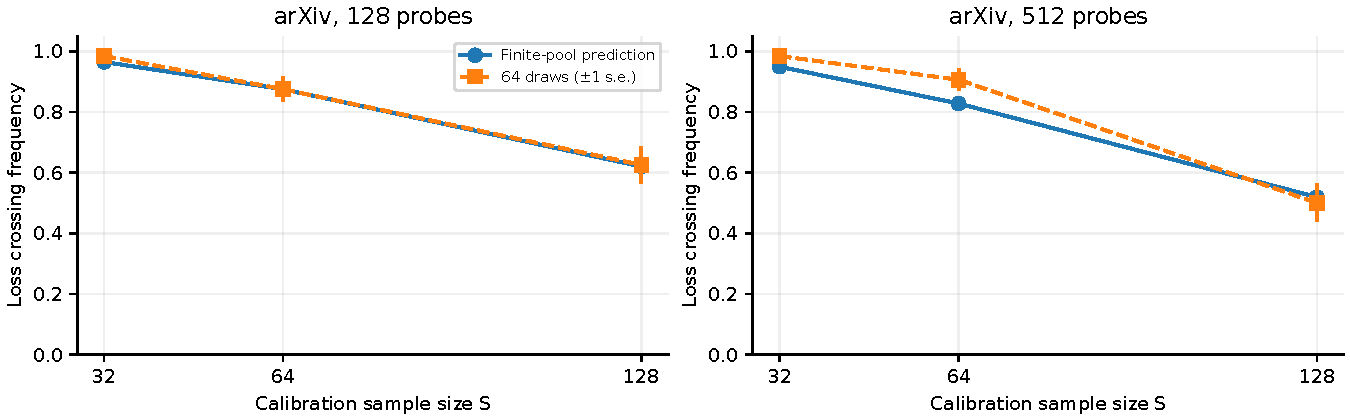
\includegraphics[width=\linewidth]{supplement/finite-pool.pdf}
\caption[Finite-pool risk prediction and observation]{Finite-pool prediction and observed arXiv loss crossings. Bars
show one estimated standard error over 64 independently drawn subsets
conditional on the fixed pool, not uncertainty over future workloads.}
\label{fig:7-finite-pool}
\end{figure}

Ten alternating repetitions resolve the apparent small-budget speed
inversion into a low-budget timing plateau. This observation does not
impose monotone runtime across all budgets and resource transitions.

\subsection{Direct calibration-plus-reuse measurement}
\label{sec:7-stream-cost}

Four cells compare fixed 64/100 with sampled and FULL calibration
over five rotated-policy rounds and 500 held-out batches. The timer
includes gathering, calibration, budget installation and first-batch graph
setup; construction, warm-up and scan calibration are excluded.
The same query pool is replayed (\cref{tab:7-stream-cost}).

\par\medskip\noindent\begin{minipage}{\linewidth}
\centering\captionsetup{hypcap=false}
\captionof{table}[Direct costs for 500 reuse batches]{Direct total milliseconds for 500 reuse batches, averaged over
five rounds, including budget calibration for sampled and FULL policies.
Each batch has 500 queries. Quality is discussed with the timing results.}
\label{tab:7-stream-cost}
\footnotesize\setlength{\tabcolsep}{4pt}
\begin{tabular}{@{}lrrrr@{}}
\toprule
Dataset/probes & Fixed 100 & Fixed 64 & Rule $S=128$ & FULL \\
\midrule
arXiv/128 & 1224 & 1102 & 1291 & 1680 \\
OpenAI-1536/128 & 1491 & 1264 & 852 & 860 \\
OpenAI-3072/128 & 2757 & 2160 & 1769 & 1783 \\
BGE/512 & 5185 & 5018 & 4921 & 5062 \\
\bottomrule
\end{tabular}

\end{minipage}\par\medskip

On OpenAI-3072/128, the sampled policy selects 4 in every round and
reduces total time from 2,757 to 1,769\,ms against fixed 100, about
36\%, at the same measured recall 0.9252. FULL selects the same budget
and takes 1,783\,ms including its larger calibration cost. On
OpenAI-1536/128, FULL takes 860 versus 1,491\,ms at the same recall
0.9280; the sampled policy averages 852\,ms and 0.9276 recall.

Measured mean cumulative savings first appear at 4/6 batches on
OpenAI-1536 and 4/9 on OpenAI-3072 against fixed 100/64
(\cref{fig:7-stream-cost}); fractional steady-rate fits are separate
model estimates. BGE/512 trades lower time for lower mean recall:
4,921 versus 5,185\,ms and 0.9658 versus 0.9670 for sampled/fixed 100.
FULL reaches 0.9664 at 5,062\,ms. ArXiv's FULL policy selects 200 for
quality and is slower than fixed 100/64, which miss the target.
Calibration's benefit therefore depends jointly on quality and total
reuse cost.

\begin{figure}[tbp]
\centering
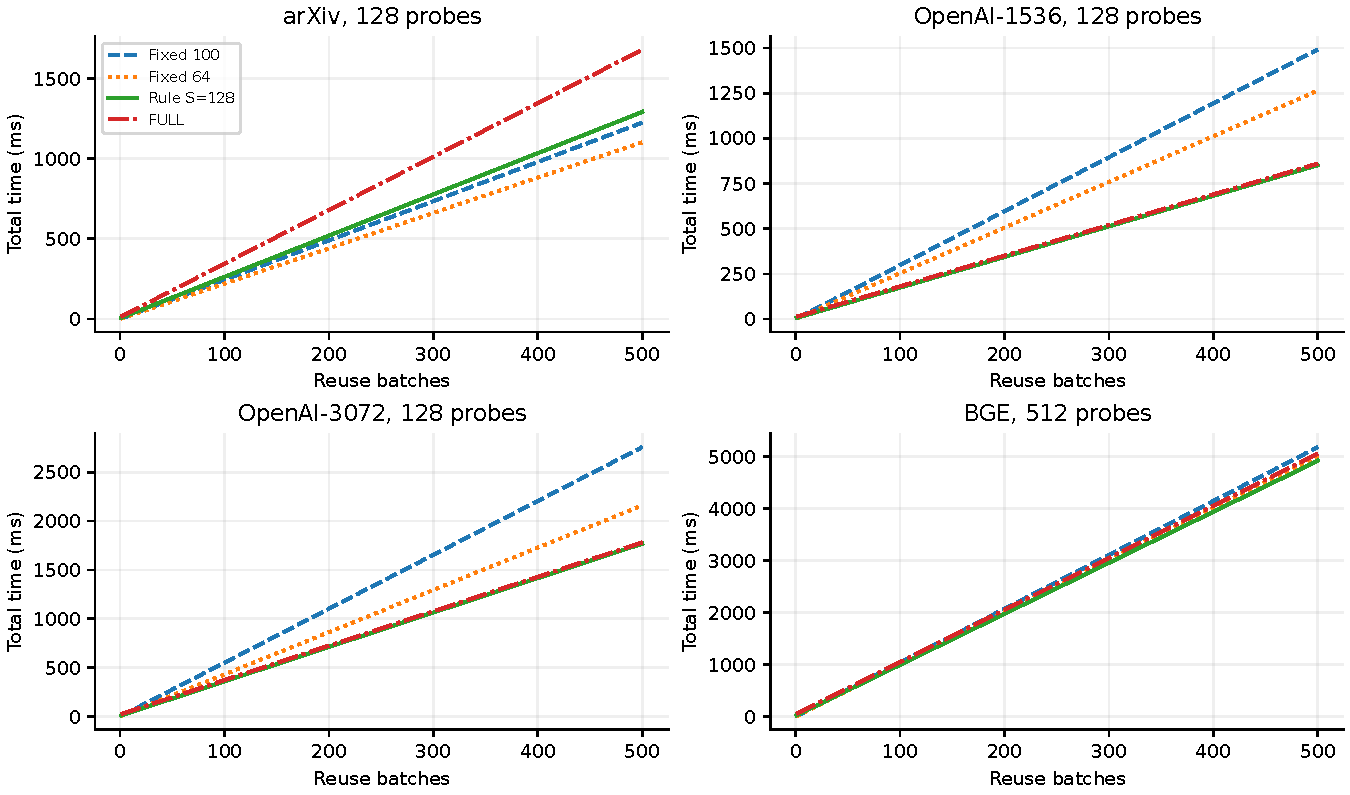
\includegraphics[width=\linewidth]{supplement/stream-cost.pdf}
\caption[Direct cumulative calibrated-reuse time]{Direct mean cumulative time, including budget calibration and
first-batch setup. Each curve replays one fixed held-out query pool.
Policies can have different recall; timings alone are not a quality-matched
ranking. Dataset/probe settings match \cref{tab:7-stream-cost}.}
\label{fig:7-stream-cost}
\end{figure}


\section{Batch Regimes, G Scheduling and Workload Skew}
\label{sec:7-6}

This section answers the performance-regime part of RQ2: when additional
scan groups supply useful parallelism, and when their extra work dominates.

\subsection{Parallelism versus repeated selection work}

For a fixed workload and timing boundary, separate scan, merge and
remaining execution time:
\begin{equation}
 \begin{aligned}
 T^{(g)}&=T_{\rm scan}^{(g)}+T_{\rm merge}^{(g)}+T_{\rm other}^{(g)},\\
 \Delta T(g)&=T^{(g)}-T^{(0)},\qquad
 T^{(g)}<T^{(0)}\iff\Delta T(g)<0.
 \end{aligned}
 \label{eq:7-group-cost}
\end{equation}
Here $g=0$ denotes the query-centric implementation and $g>0$ a grouped
path. The three time categories are disjoint: staging and local
selection already included in scan time are not charged again.
This is an accounting identity, not an analytical latency predictor.

At batch 8, one block per query exposes only eight blocks on 170 SMs.
Eight scan groups improve end-to-end throughput by $2.06$--$2.76\times$.
For example, arXiv's scan falls from 849 to 216\,$\mu$s while merging
adds 16.7\,$\mu$s. At batch 1,000, arXiv with $\alpha=200$ instead
increases scan time from 3,530 to 7,652\,$\mu$s and adds
2,624\,$\mu$s of merging; the independent-bound path reaches only
about $0.46\times$ its one-block throughput. Extra parallelism repays
its duplicated work in the first regime and loses in the second.
Shared bounds reduce work without removing this regime change.

\begin{figure}[tbp]
\centering
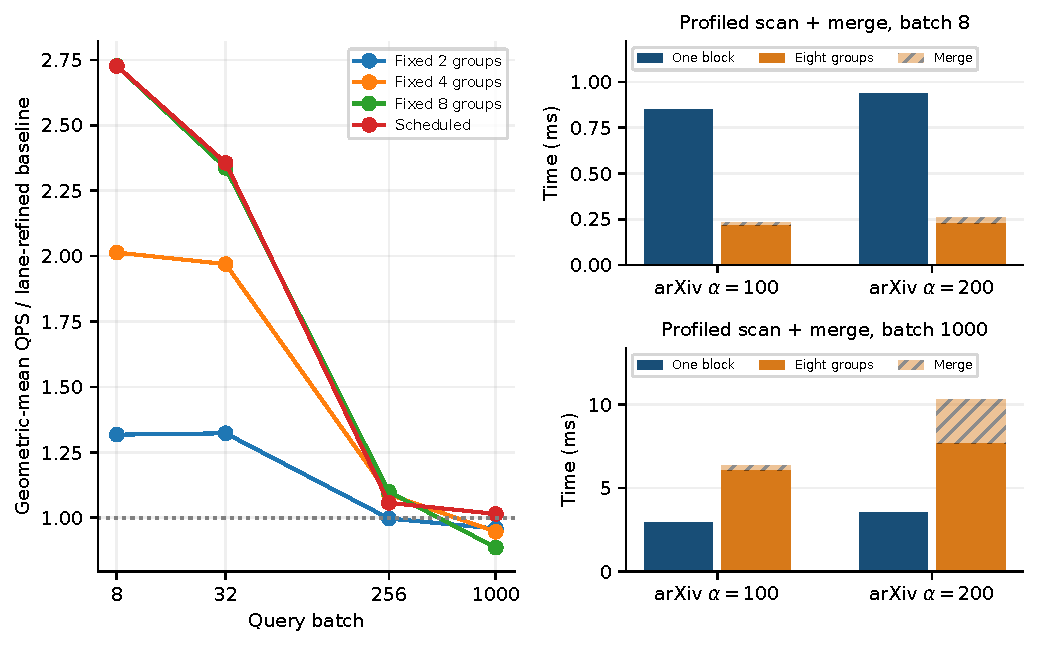
\includegraphics[width=\linewidth]{ch7/batch_execution.pdf}
\caption[Batch-dependent execution regimes]{Execution regimes. Left: fixed shared-bound group counts and
scheduled execution relative to the lane-refined one-block baseline
(13 cells at small batches, 11 at batch 1,000). Right: paired scan and
merge profiles at batches 8 and 1,000 for arXiv budgets 100 and 200.
Hatching denotes merge time. The right panels use the independent-bound
scan experiment; they explain a cost, not the scheduler's entire speedup.}
\label{fig:7-batch}
\end{figure}

\subsection{A fixed rule evaluated on further configurations}

The scheduler follows the fill/skew rule and pseudoquery calibration
in \cref{sec:5-5}. Four configurations set the constants before the
additional configurations were measured.


\begin{table}[tbp]
\centering
\caption[Integrated execution and scheduling gains]{Integrated execution gains over v61 L16. Entries are geometric
 means of per-cell median paired speedups from five rounds. ``Held out''
 excludes the four configurations used to set the rule; it means held-out
 configurations, not the budget experiment's held-out query split.}
\label{tab:7-scheduling}
\small\setlength{\tabcolsep}{4pt}
% Generated by scripts/build_ch7.py; do not edit numbers manually.
\begin{tabular}{@{}rrrrrrr@{}}
\toprule
Batch & Cells & $g_s=2$ & $g_s=4$ & $g_s=8$ & Scheduled & Held out \\
\midrule
8 & 13 & 1.318 & 2.014 & 2.728 & 2.727 & 2.930 \\
32 & 13 & 1.323 & 1.970 & 2.337 & 2.356 & 2.560 \\
256 & 13 & 0.997 & 1.090 & 1.099 & 1.057 & 1.041 \\
1000 & 11 & 0.959 & 0.947 & 0.886 & 1.015 & 1.012 \\
\bottomrule
\end{tabular}

\end{table}

\Cref{tab:7-scheduling} gives the paired gains and evaluation subsets.
The small-batch means use thirteen configurations; batch 1,000 uses
eleven because Stella has 999 queries, with nine/seven held-out
configurations respectively. Scheduling retains the batch-8 benefit
while protecting full-batch execution: fixed eight groups fall to
$0.886\times$ at batch 1,000. The largest scheduler regret is
1.217 on BGE at batch 256, showing that candidate-count CV omits
some traversal and selection costs.

Vogue illustrates both the value and limits of the skew feature. Its E1
candidate-count CV ranges from 0.338 to 0.622 as probes change, forcing
four groups at batch 1,000. The integrated path/one-block ratio ranges
from 0.895 to 1.175. It loses at $(n_{\rm probe},\alpha)=(16,16)$,
$(16,64)$ and $(32,64)$, with ratios 0.955, 0.895 and 0.955.
Candidate-count dispersion alone does not encode absolute per-query work;
the rule can add overhead to these low-probe cases while enabling Vogue's
0.97 cross-system lead in \cref{sec:7-2}. Both failures expose
decomposition costs missing from the CV feature.

Finally, correctness is checked independently of timing. Across 250
variant/configuration comparisons and 234,320 query comparisons, the
integrated campaign reports no non-tie primary-selection differences and
no different final identifier sets. Final order can differ at ties;
the entire campaign should not be described as universally bit-identical.
The throughput results concern sequential, synchronous submissions and
do not establish tail latency under an open-loop arrival process.

\section{Cold Construction, Resident Memory and Tested Scale}
\label{sec:7-7}

RQ1 is assessed through cold construction, resident memory and completed
large-dataset searches; the E1 memory comparison also informs RQ4.

\subsection{Cold builds and the lifecycle boundary}

Unlike the cached search sweeps, \cref{tab:7-build-memory} uses three
normal empty-cache train/add repetitions per dataset.
Vogue's training is 298--303\,ms, so its normal total is about 0.56\,s;
the archived 1.33\,s total (including 1.056\,s training) is an unusually slow single observation.
Stella's normal totals are 10.54--10.65\,s, close to the historical
10.40\,s record.

\begin{table}[tbp]
\centering
\caption[Cold construction and resident memory]{Cold JHQ construction and separately measured resident memory.
Train/add are component medians of three supplementary normal builds;
Total is the median paired sum. Memory comes
from v71's two-group, 128-probe, $\alpha=100$ runs and includes context
and workspace. ``Residual'' is the modelled residual-code share of the
measured used total, not the fraction read per query.}
\label{tab:7-build-memory}
\small\setlength{\tabcolsep}{3pt}
% Generated by scripts/build_ch7.py; do not edit numbers manually.
\begin{tabular}{@{}lrrrrrr@{}}
\toprule
Dataset & Train s & Add s & Total s & Used GiB & Raw GiB & Residual \\
\midrule
Vogue & 1.06 & 0.27 & 1.33 & 1.47 & 2.67 & 45.4\% \\
arXiv & 0.59 & 0.52 & 1.10 & 2.58 & 6.45 & 62.5\% \\
OpenAI-1536 & 0.64 & 0.38 & 1.01 & 2.39 & 5.72 & 59.7\% \\
OpenAI-3072 & 1.34 & 0.65 & 1.99 & 4.14 & 11.43 & 69.0\% \\
BGE & 3.75 & 3.67 & 7.42 & 11.93 & 38.50 & 80.7\% \\
Stella & 3.74 & 6.67 & 10.40 & 20.44 & 67.81 & 82.9\% \\
\bottomrule
\end{tabular}

\end{table}

Construction and startup boundaries follow \cref{sec:3-3,sec:a-e1-protocol};
\cref{fig:7-build} compares these repetitions with baseline configurations.


\begin{figure}[tbp]
\centering
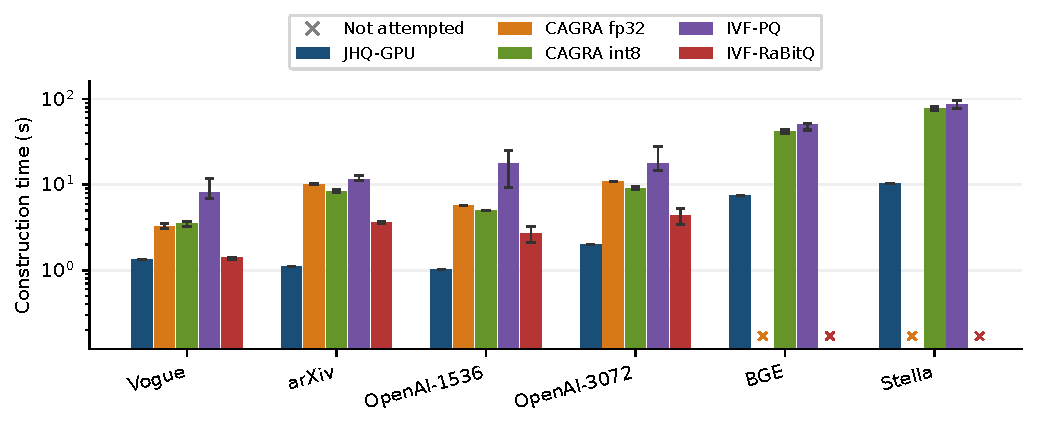
\includegraphics[width=\linewidth]{ch7/construction.pdf}
\caption[Recorded construction costs]{Recorded construction costs, with CAGRA int8 included. JHQ is
the median and range of three supplementary normal cold builds with warm
input pages; other bars are medians across successful
measured index configurations, with minimum--maximum whiskers. Int8
includes dataset quantization; RaBitQ excludes the required serialization
round trip. Missing large-dataset bars denote unattempted configurations,
not measured build failures. The vertical axis is logarithmic.}
\label{fig:7-build}
\end{figure}

On Stella, successful isolated CAGRA int8 builds take approximately
74.55 and 82.45\,s including dataset quantization, depending on graph
degree; the measured IVF-PQ build median is 86.59\,s across its three
configurations. JHQ's 10.54--10.65\,s repeated interval is substantially shorter under the
reported boundaries. Downstream quality and resident cost are evaluated
separately.


Five independent builds give a maximum fixed-point recall range
of 0.0012 on arXiv; normal timing uses three uninstrumented builds.
Startup is a broader boundary: Stella takes 18.2--18.6\,s with warm
input pages, versus 129.9\,s on the session-first read.
Twenty-millisecond device sampling observes 26.08\,GiB near BGE's
add entry and 22.58\,GiB during Stella's repack. BGE's three
assignment buffers total 12\,GiB in an earlier lifetime than the
23.05\,GiB gather payload (\cref{eq:4-assignment-scratch}); the two
allocations must not be summed as a simultaneous peak.

\subsection{Resident allocation and where compression helps}

\Cref{fig:7-memory} combines the component model in \cref{sec:4-4}
with measured resident totals. Its unattributed remainder is retained,
and the preceding construction measurements give the sampled peaks.


\begin{figure}[tbp]
\centering
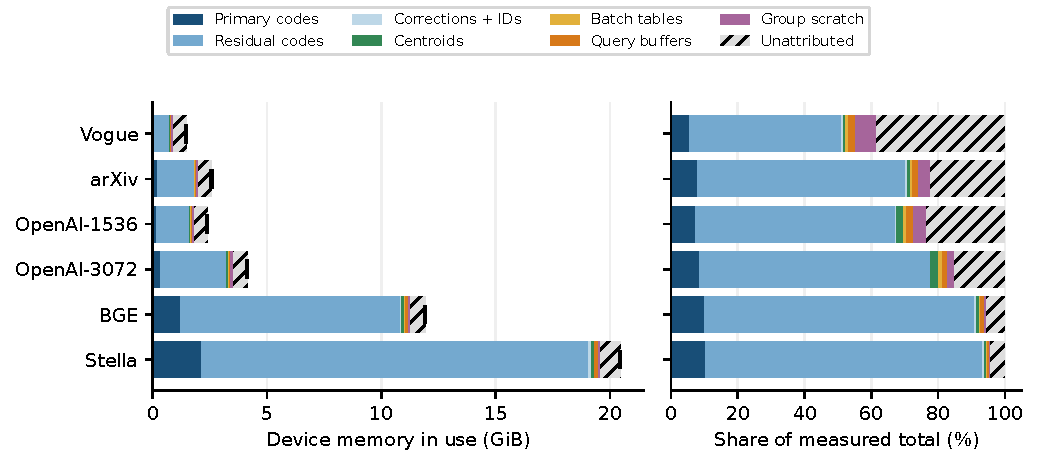
\includegraphics[width=\linewidth]{ch7/memory.pdf}
\caption[Resident-memory decomposition]{Resident-memory decomposition at two-group tables, 128 probes
and $\alpha=100$. Component sizes are modelled, markers are measured used
totals, and hatching is the unattributed remainder. The totals include
context and workspace. The preceding construction measurements give sampled peaks; these
resident markers are not peaks.}
\label{fig:7-memory}
\end{figure}

Residual codes account for 80.7\% of BGE's 11.93\,GiB and 82.9\%
of Stella's 20.44\,GiB measured totals. Raw FP32 vectors alone would
require 38.50 and 67.81\,GiB. These resident totals include context
and query workspace; lowering $\alpha$ changes residual access rather
than the stored array. The component model is in \cref{sec:4-4}.

The reserved group workspace is about 93.8\,MiB even on the one-block
path, for batch capacity 1,024 and up to eight groups. Actual group
count therefore does not determine allocated capacity. Construction
peaks and after-build index deltas also exclude different allocations;
some baseline search pools are initialised after index-memory measurement.

The E1 measurements provide a separate cross-system view in
\cref{tab:7-e1-memory}. Subtracting the baseline-measured 507.2\,MiB
context from JHQ's process total gives approximately 0.29--0.39 of
CAGRA fp32's index allocation. JHQ's figure includes workspace, whereas
CAGRA's is the build-time index delta. These are parameter-sweep ranges,
not memory-matched recall points or a comparison of equal peak budgets.
The CAGRA int8 allocations in the same table are of a similar order to
JHQ's: compression relative to fp32 is shared by competing designs.
The component model in \cref{tab:4-bytes} explains this comparison.

\begin{table}[tbp]
\centering
\caption[E1 allocation ranges]{E1 allocation ranges. JHQ is process total minus a 507.2\,MiB
context estimate, including query workspace; both CAGRA columns are index
allocations measured during build. Ranges cover the parameter sweep.}
\label{tab:7-e1-memory}
\footnotesize\setlength{\tabcolsep}{4pt}
% Generated by scripts/build_ch7.py; do not edit numbers manually.
\begin{tabular}{@{}lrrr@{}}
\toprule
Dataset & JHQ net process GiB & CAGRA fp32 index GiB & Ratio range \\
\midrule
Vogue & 0.90--1.01 & 2.89--2.91 & 0.31--0.35 \\
arXiv & 2.01--2.19 & 6.84--6.98 & 0.29--0.32 \\
OpenAI-1536 & 1.79--2.33 & 5.95--5.97 & 0.30--0.39 \\
OpenAI-3072 & 3.54--3.82 & 11.67--11.68 & 0.30--0.33 \\
\bottomrule
\end{tabular}

\end{table}

\subsection{Large-dataset feasibility and competitive regions}

BGE contains 10,091,524 vectors and Stella 17,776,615, both with
1,024 dimensions and 32,768 IVF lists. Stella's queries are sampled from
the corpus; its result therefore characterizes that benchmark rather
than an independently collected external-query distribution.
\Cref{fig:7-large} includes
successful CAGRA int8 and IVF-PQ measurements. Full-precision CAGRA,
RaBitQ configurations and FP32 brute force were not attempted in the
large-scale comparison when their computed storage requirements exceeded
the available device capacity. Those omissions are planned feasibility
exclusions, not observed out-of-memory errors or measured recall failures.

\begin{figure}[tbp]
\centering
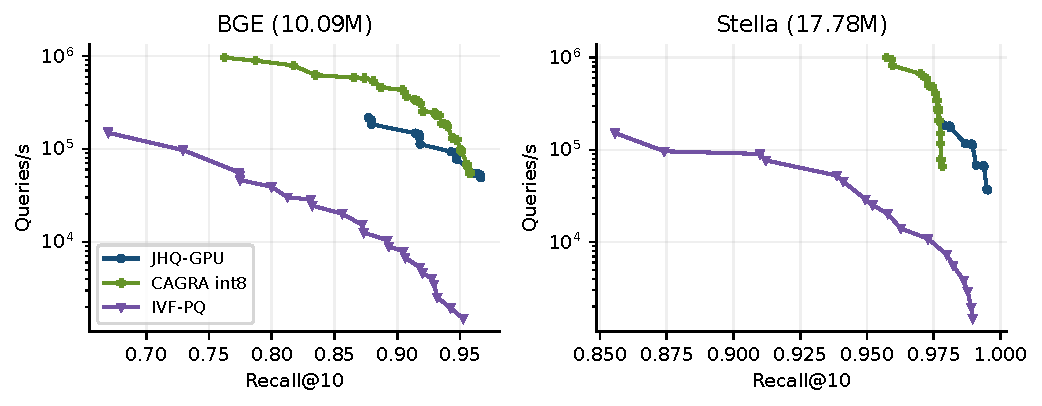
\includegraphics[width=\linewidth]{ch7/large_frontiers.pdf}
\caption[Large-dataset search frontiers]{Large-dataset host-to-host frontiers, including the successful
isolated CAGRA int8 reruns. BGE uses 1,000 queries and Stella 999. An
endpoint is the end of the tested grid, not an intrinsic recall limit.}
\label{fig:7-large}
\end{figure}

Successful isolated reruns show that CAGRA int8 fits Stella in the
tested configurations. On BGE, int8 is approximately $1.35$--$2.96\times$
faster at the sampled common targets 0.88/0.90/0.92/0.94/0.95. At its
measured maximum recall 0.9579, JHQ's interpolated QPS is $1.086\times$
int8's. Thus the advantage changes direction near the high-recall end.
The maximum tested recalls are 0.9579/0.9783 for int8, 0.9663/0.9952
for JHQ and 0.9525/0.9896 for PQ on BGE/Stella.

On Stella, one concrete high-end comparison is 185.4 kQPS at recall
0.978679 for JHQ versus 66.3 kQPS at 0.978278 for int8, a $2.80\times$
rate ratio with slightly different recall. This is an explicit pair of
measured points, not a uniform matched-recall gain: much of JHQ's
higher-recall region has no int8 coverage, and JHQ's highest-recall
points trade throughput for quality. Corrected-run exclusions and
harness diagnostics are recorded in Appendix~\ref{app:reproducibility}.

The experiments demonstrate single-GPU search over 17.78 million vectors
and useful high-recall operating regions. Multi-GPU execution and
scaling at a fixed data distribution remain untested. Construction
memory samples leave shorter allocation transients unresolved near
device capacity. Stella uses its actual 999-query pool.

\section{Numerical Robustness, Anomalies and Recall Attribution}
\label{sec:7-8}

The robustness checks qualify the RQ2 exactness claims, the RQ3 risk
assessment and the small cross-system margins in RQ4.

\subsection{Quality resolution and repeated execution}

With $k=10$ and 1,000 queries, one recovered neighbour changes aggregate
Recall@10 by $10^{-4}$; with 500 held-out queries the resolution is
$2\times10^{-4}$. Stella's 499-query split has a slightly coarser
resolution. This discretization is not an uncertainty interval, but it
helps interpret the small differences reported above. A fourth-decimal
change may represent only one or two result slots, while a small mean
loss can still hide several queries with substantially changed answers.

Repeated calls and repeated index builds answer different questions.
E1 retains 369 baseline repeat-call identifier flags, including tie-order
changes; these points remain in the frontiers. The 401-count convention
and cross-protocol checks are separated in \cref{sec:a-e1-protocol}.

Five-round ranges describe timing within a fixed build. A separate
frontier-slope calculation quantifies sensitivity to a horizontal recall
shift: continuous log-QPS segments adjacent to 0.97 imply about
1.01--3.17\% rate change per $10^{-3}$ recall, before applying the
near-target snapping convention. The supplementary five-build recall ranges are 0.0008 for Vogue,
0.0012 for arXiv, 0.0004 for OpenAI-1536 and 0.0002 for OpenAI-3072
at fixed operating points. Applied purely as horizontal sensitivity
scales to the local slopes, these imply changes of order a few percent,
rather than the larger OpenAI fp32-CAGRA margin. The experiment does
not repeat whole frontiers or baseline builds; it therefore supports
local stability assessment, not a universal bound on matched ratios.
The precision intervention in \cref{sec:7-precision} directly establishes
that the OpenAI advantage survives removal of TF32 under its stated
cached-model boundary. ArXiv and the LUT near ties retain their narrower
interpretation.

Across each dataset's RaBitQ configurations, the median five-round
range divided by median QPS is 3.79\%, 3.34\%, 2.87\% and 5.25\%
for Vogue, arXiv, OpenAI-1536 and OpenAI-3072. These descriptive spreads
are comparable in scale to the small Vogue advantage, rather than
confidence intervals for its matched ratio. Raw call traces also contain
long calls, including occasional 30--60\,ms observations in otherwise
faster configurations. As a sensitivity check, recomputing QPS as
$10^6/\operatorname{median}(\text{call latency in ms})$ for a
1,000-query call reduces the influence of long calls.
At recall 0.97, the resulting JHQ/RaBitQ ratios are 1.063, 0.995,
1.118 and 1.100. The three favourable directions and arXiv near parity
remain, so the result is not solely a consequence of long calls.

\subsection{Exactness is attached to a particular stage}
\label{sec:7-recall-attribution}

The stage contracts in \cref{tab:5-query-stages} distinguish computed-score
selection from raw-space kNN; lane rounding, cutoff ties and process
variation qualify different stages.


The archived reconstruction pilot measures the remaining gap to
full-probe reconstructed scoring.
Across seven workload--budget arms of 128 queries each, scoring all
probed candidates in FP64 improves recall over GPU outputs at selected budgets by
0--0.002344. For arXiv at 128 probes, $\alpha=200$ matches the full-IVF
reconstructed answer set on all 128 queries. At 100, the recall is
0.9734375 versus 0.9750 for full-IVF scoring: an additional 0.0015625
budget deficit beside the joint routing/reconstruction deficit of
0.0250 (\cref{sec:6-2}). These are pilot-specific aggregate differences;
the seven arms include two budgets on one dataset--probe workload.
FP64 reconstructed scoring also differs from the GPU arithmetic, so the
pilot does not isolate a pure budget effect in every arm. Separating
routing from representation requires additional stage-wise GT coverage.
